 \documentclass[dvipsnames]{beamer}%[trans] for handouts
%\usepackage[letterpaper,margin=.5in,foot=0in]{geometry}
 
 %\usepackage[T1]{fontenc}

\usepackage[sort]{natbib}
\bibliographystyle{apa}
	\bibpunct[:]{(}{)}{,}{a}{}{,}

\usepackage{stmaryrd}
\usepackage{amsmath,nccmath} 

 \usepackage{textcomp}
 \usepackage{ragged2e}
 \usepackage{booktabs,colortbl}
% \usepackage{newtxmath,newtxtext}
\usepackage{xltxtra}

\usepackage{graphicx}

 \usepackage{comment}
 \defaultfontfeatures{Mapping=tex-text}
 %\setromanfont[Mapping=tex-text]{Hoefler Text}
 %\setsansfont[Scale=MatchLowercase,Mapping=tex-text]{Gill Sans}
 %\setmonofont[Scale=MatchLowercase]{Andale Mono}
 
\usepackage{wrapfig}
 \setmainfont{Cambria}
\makeatletter
\def\@xfootnote[#1]{%
	\protected@xdef\@thefnmark{#1}%
	\@footnotemark\@footnotetext}
\makeatother

 

 \pagenumbering{gobble}
% \usepackage{subcaption}
% \captionsetup{compatibility=false}
 \usepackage{amsthm}
 \usepackage[normalem]{ulem}
 \usepackage{amssymb}
 \usepackage{multirow}
 \usepackage{mathrsfs}
 \usepackage{pifont}
 \usepackage{mathtools}
 \usepackage{tikz}
% \usepackage{qtree}
 \usepackage{tikz-qtree}
 %\usepackage{tipa}
 \usetikzlibrary{decorations}
 \usetikzlibrary{decorations.pathreplacing}
 \usepackage{textcomp}
 \usepackage[normalem]{ulem}
 \usepackage{url}
 \usepackage[all]{xy}
 \usepackage{multicol}
 \usepackage{hanging}
 \usepackage{booktabs}
 \usepackage{setspace}
 \usetikzlibrary{shapes,backgrounds}
% \usepackage{geometry}
 
 
 
 % \newtheorem{definition}{Definition}
 %\newtheorem{theorem}{Theorem}
 
 
 \usepackage{enumerate}
 %\usepackage{gb4e} \let\eachwordone=\sl
 \usepackage{expex}	
	 \lingset{exnoformat={\bf\it X},labelformat={\bf\it A},labeloffset=0.05em,aboveexskip=.5ex,belowexskip=.5ex,aboveglftskip=.55ex}
	 \lingset{textoffset=.8em,everytrailingcitation=\footnotesize}
 
 
 
 %\newcommand{\denote}[1]{\mbox{$[\![\mbox{#1}]\!]$}}
 \newcommand{\concat}{\mbox{$^\frown$}}
 \newcommand{\ph}{\varphi}
 \newcommand{\vsep}{\vspace{8pt}}
 \newcommand{\linesep}{\rule{6.5in}{.5pt}}
 \def\attop#1{\leavevmode\vtop{\strut\vskip-\baselineskip\vbox{#1}}}
\providecommand{\denote}[2][]{\ensuremath{\llbracket{#2}\rrbracket^{#1}}}
 \newcommand{\exref}[1]{~(\ref{#1})}
 \newcommand{\glem}[1]
 {\MakeUppercase{\scriptsize{\textbf{#1}}}}
  \newcommand{\textbc}[1]
  {\MakeUppercase{\footnotesize{\textbf{#1}}}}
 \newcommand{\la}{\langle}
 \newcommand{\ra}{\rangle}
 \newcommand{\lamda}{\lambda}
 \definecolor{ochre}{cmyk}{0, .42, .83, .20}
 \definecolor{forest}{cmyk}{.64, .03, .97, .68}
 \definecolor{maroon}{cmyk}{0, 1, .07, .5}
 \definecolor{plum}{cmyk}{.48,.85,.29,.2}
 \definecolor{peri}{cmyk}{.2,.2,0,0}
 \usepackage{framed}
 %\usetheme{Warsaw}
 %\usecolortheme{wolverine}
 \setbeamercolor{frametitle}{bg=violet!60,fg=black}
 \setbeamercolor{title}{bg=violet!60,fg=black}
 \setbeamercolor{palette sidebar primary}{use=normal text,fg=normal text.fg}
 
 %\input{setup}
 
 %\singlesidestandardsetup
 
 %\parindent 1em
 
 %\input{psfig-scale}
 
  \newcommand{\I}{\textbf{\textcolor{forest}{I}}}
   \newcommand{\II}{\textbf{\textcolor{ochre}{II}}}
    \newcommand{\III}{\textbf{\textcolor{blue}{III}}}
     \newcommand{\IV}{\textbf{\textcolor{violet}{IV}}}
 
 
% \newcommand{\verteq}{\rotatebox{90}{$\,=$}}
% \newcommand{\equalto}[2]{\underset{\scriptstyle\overset{\mkern4mu\verteq}{#2}}{#1}}
 
 
% \newcommand{\secsep}{\hrulefill}
 % \renewcommand*{\marginfont}{\small}
 \usepackage{qtree}
% \qtreecenterfalse
 
% \renewcommand{\baselinestretch}{1.2} 
 \usepackage{xcolor}
 \definecolor{dgreen}{rgb}{0.,0.6,0.}
 


 \definecolor{ochre}{cmyk}{0, .42, .83, .20}
 \definecolor{forest}{cmyk}{.57, .13, .57, .08}
 \definecolor{maroon}{cmyk}{0, 1, .07, .5}
 \definecolor{peri}{cmyk}{.2,.2,0,0}
 \definecolor{yale}{cmyk}{1,.75,.08,.4}
 \usepackage{framed}
 
  \title[]{\textbf{Reality status \& the Yolŋu verbal paradigm}}
  \subtitle{A formal account of an irrealis mood}
  \author{Josh Phillips{\scriptsize\\\texttt{josh.phillips@yale.edu}}}
  \institute{\textcolor{yale}{Yale Linguistics}}
  \date[FoDS4]{\footnotesize{\textcolor{violet}{\textit{Dissertation defense}\\\scriptsize{21 December 2020}}}}

\useoutertheme{smoothbars} %sidebar,split or smoothbars are also options
\usefonttheme[stillsansserififlarge,stillsansserififsmall]{serif}
		\addtobeamertemplate{navigation symbols}{}{%
			\usebeamerfont{footline}%
			\usebeamercolor[fg]{footline}%
			\hspace{1em}%
			{{\color{ochre!50}\small\textbf{\insertframenumber}}}
		}
		
\resetcountonoverlays{excnt}


\begin{document}


\frame[noframenumbering]{\titlepage}



\begin{frame}{Roadmap}
	\tableofcontents
\textsf{}\end{frame}
\section{introduction}
\subsection[TAM prominence]{the notion of TAM prominence}
	\begin{frame}{\textbf{Introduction}\hfill TAM prominence}
		\begin{columns}[c]
			\column{.65\textwidth}
			\begin{itemize}
				\item<1-> As I've suggested, \textsc{tense, mood, aspect} are related categories
				\item<2-> Bhat's typological claim (1999): \textit{languages can be regarded as \textsc{tense-, aspect-} or \textsc{mood-}\textbf{prominent}}
				%I.e. languages afford a particularly priveleged status to one of these categories. Other categories are often understood in terms of the ``prominent'' category.
%				\item Correlations between hypothesised \textsc{types} and other features of the grammar
%				%e.g. a lack of stative verbs in T-prom langs, grouping of adjectival with nouns...

								%to the extent that this claim is borne out...
				\item<3-> Typology implies • conceptual connections between categories • and that languages can `move between' these ``types''. 
			
			
			\item<4-> Cross-categorial change between \textbf{\textcolor{red}{tense}, \textcolor{blue}{modal}, \textcolor{forest}{aspectual}} domains {\scriptsize(Bybee \textit{et al.} 1994; Condoravdi \& Deo 2014)}\\
	\begin{tikzpicture}[baseline=-2pt]
				\draw  (0,0) node(pf)  {\textcolor{forest}{\textsc{perf}}};
				\draw (1.75,.5) node(pv) {\textsc{pfv}};
				\draw (1.75,-.5) node(ps)  {\textcolor{red}{\textsc{pst}}};
				\draw[thick,->] (pf) -- (ps);
				\draw[->] (pf) -- (pv);
			\end{tikzpicture}\hfill
			\begin{tikzpicture}[baseline=-2pt]
				\draw  (0,0) node(pg)  {\textcolor{forest}{\textsc{prog}}};
				\draw (1.75,.5) node(ip) {\textsc{ipfv}};
				\draw (1.75,-.5) node(pr)  {\textcolor{red}{\textsc{pres}}};
				\draw[->] (pg) -- (ip);
				\draw[thick, ->] (pg) -- (pr);
			\end{tikzpicture}
			
%			\onslide<3->{
%				\item \textit{This} implies conceptual links between temporal, modal \& aspectual categories
								
			\end{itemize}
			\onslide<2->{\column{.32\textwidth}
			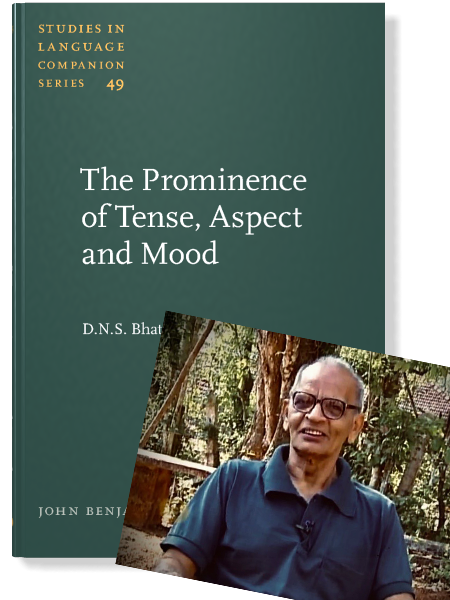
\includegraphics[width=1.125\textwidth]{bhat-bk.png}}
		\end{columns}
	\end{frame}


%\begin{frame}{\textbf{Introduction}\hfill Semantic change in the TAM domain}
%\begin{itemize}
%\item `Paths of semantic evolution for grammatical forms are constrained and trajectorial.' {\scriptsize(Deo 2015)}
%\
%
%\item Analyses of ``future tense'' as a modal operator 
%
%\end{itemize}
%\end{frame}


\begin{frame}{Branching times}
\textbf{\textit{if the determinist sees Time as a line, the indeterminist sees it as a system of forking paths\hfill} Burgess '78}

	\begin{columns}
\column{.6\textwidth}\begin{itemize}
%	\item Even if a grammar lends particular ``prominence'' to one of these categories, all natural language can talk about temporal/aspectual/modal concepts (ofc) 
	\item Futurity as a modal concept {\scriptsize (Abusch 1985, Copley 2004, Kaufman 2005, Giannakidou 2012...)}
	 \item Manipuri \textit{li} \textsc{\textcolor{red}{`fut'}} $ \boldsymbol\leftarrow$ \textsc{\textcolor{blue}{`irr'}} (\textit{e.g.},~Mao~Naga \textit{le})\\{\scriptsize(Bhat 1999: 19,67,183)}
\end{itemize}
\column{.4\textwidth}
\begin{figure}[h]
	\centering
	\begin{tikzpicture}
		[scale=1.1,level distance=9mm,
		every node/.style={fill=black,circle,inner sep=1.5pt},
		level 1/.style={sibling distance=10mm},
		level 2/.style={sibling distance=8mm},
		level 3/.style={sibling distance=4mm},
		level 4/.style={sibling distance=2mm},
		edge from parent/.style={draw}]
		\node {} [grow=right]
		child {node {} edge from parent[densely dotted]
			child {node {}
				child {node {}
					child {node {}}
					child {node {}}}
				child {node {}
					child {node {}}
					child {node {}}}}
			child {node {}
				child {node {}
					child {node {}}
					child {node {}}}
				child {node {}
					child {node {}}
					child {node {}}}}}
		child[missing]
		child {node {}
			child {node {} edge from parent[densely dotted]
				child {node {}
					child {node {}}
					child {node {}}}
				child {node {}
					child {node {}}
					child {node {}}}}
			child {node {} edge from parent[densely dotted]
				child {node {}
					child {node {}}
					child {node {}}}
				child {node {}
					child {node {}}
					child {node {}}}}
			child {node [style={fill=red},label=above:$ \boldsymbol{i*} $] {}
				child {node {} edge from parent[densely dashed]
					child {node {}}
					child {node {}}}
				child {node {} edge from parent[densely dashed]
					child {node {}}
					child {node {}}}}};
\end{tikzpicture}\end{figure}

\end{columns}
\end{frame}
%
%\begin{frame}{\textbf{Introduction}\hfill Mood-based inflection}
%\begin{itemize}
%	\item Krifka's (2016) proposal for the Daakie inflectional system\\
%\pause\begin{itemize}
%	\item \textsc{realis}
%	\item \textsc{realis negation}
%	\item \textsc{potentialis}
%	\item \textsc{potentialis negation}
%	\item \textsc{distal}
%\end{itemize}\pause
%\item Nonfuture (anti)factivity presupposition in \textsc{realis} categories
%\item \textsc{potentialis} existentially quantify over future indices
%\begin{itemize}
%	\item co-occur with non-realis Cº, taken to introduce conversational backgrounds
%\end{itemize}
%
%\end{itemize}
%\end{frame}
%
%\section[Language background]{Language background}
%\begin{frame}{\textbf{Australia}\hfill Language background}
%	\begin{columns}
%		\column{.45\textwidth}
%		\begin{itemize}
%			\item 50,000y archæological record
%			\item ca. 360 languages spoken at European contact
%			\item 275 ``Pama-Nyungan'' languages
%		\end{itemize}
%		\column{.55\textwidth}
%%		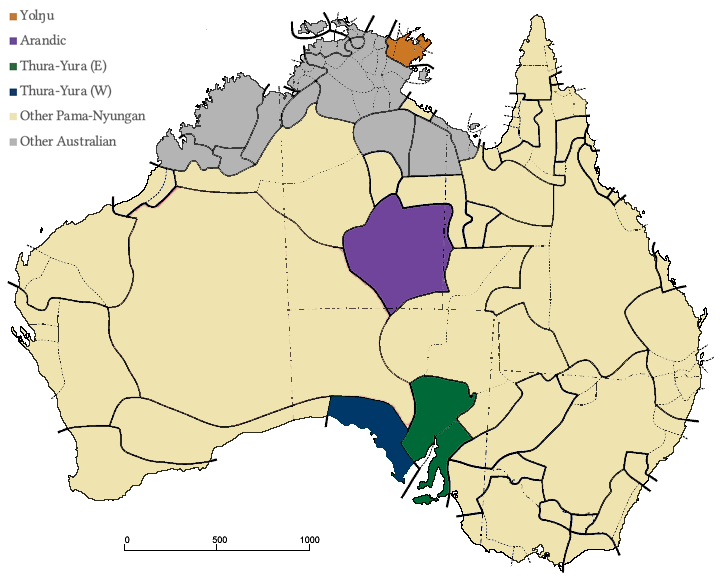
\includegraphics[scale=.33]{YolTYAr}
%	\end{columns}
%\end{frame}
%\subsection[Yolŋu]{Yolŋu~Matha: an expanding domain}



%
%\begin{frame}{\textbf{Yolŋu}\hfill Language background}
%\begin{columns}
%\column{.75\textwidth}
%	\begin{itemize}
%		\item 5-6 languages
%		\item 30+ `clan-lects'
%		\item ca. 5000 speakers
%	\end{itemize}
%\hspace*{\fill}\column{=.25\textwidth}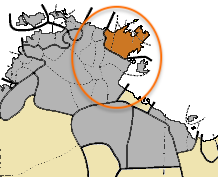
\includegraphics[scale=.55]{Arnhem}
%\end{columns}
%	
%	\includegraphics[scale=.2]{Phylo}
	
	%\begin{tikzpicture}	\tikzset{edge from parent/.style=
	%	{draw,
	%		edge from parent path={(\tikzparentnode.south)
	%			-- +(0,-8pt)
	%			-| (\tikzchildnode)}}}
	%\tikzset{frontier/.style={distance from root=90pt}}
	%
	%\Tree [.{\bf{\it{\sc Yolŋu~Matha}}} [.{\it Western} Djinaŋ Djinba ] [.{\it Northern} Nhaŋu [ Dhaŋu Djaŋu ] ] [.{\it Southern} [.Dhuwal(a) \textbf{\textsc{west}} \textsc{east} ] [ \textbf{Ritharrŋu~Wägilak} ] ] ] 
	%
	%\end{tikzpicture}
%	
%\end{frame}
%
%
%
%\begin{frame}{\textbf{Yolŋu}\hfill Language background}
%	\begin{columns}
%		\column{.5\textwidth}
%		\begin{itemize}
%	\item Strict exogamy, stable language contact/variation
%	\item A Pama-Nyungan `enclave' -- bordered by families of unrelated languages
%		\end{itemize}
%		\column{.5\textwidth}
%
%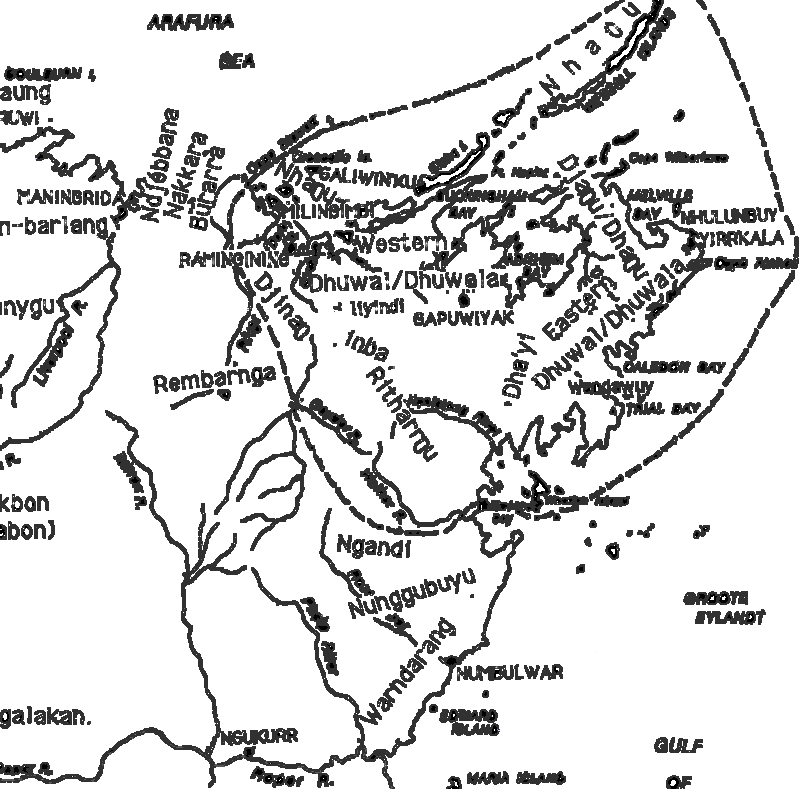
\includegraphics[scale=.36]{YolnguWanga-MW}
%	\end{columns}
%%	\framezoom<1><2>(.3cm,.3cm)(1cm,1.5cm)
%\end{frame}

\begin{frame}{\textbf{Yolŋu}\hfill Verbal morphology}
\begin{columns}
\column{0.5\textwidth}


	\begin{itemize}
	\item Significant variation in grammatical expression of TMA
	\item Cognate inflectional paradigms point to semantic change
	\item \textbf{Djambarrpuyŋu} and \textbf{Wägilak}: all verbs inflect for four categories
 	\end{itemize}
 		\column{.5\textwidth}
 
 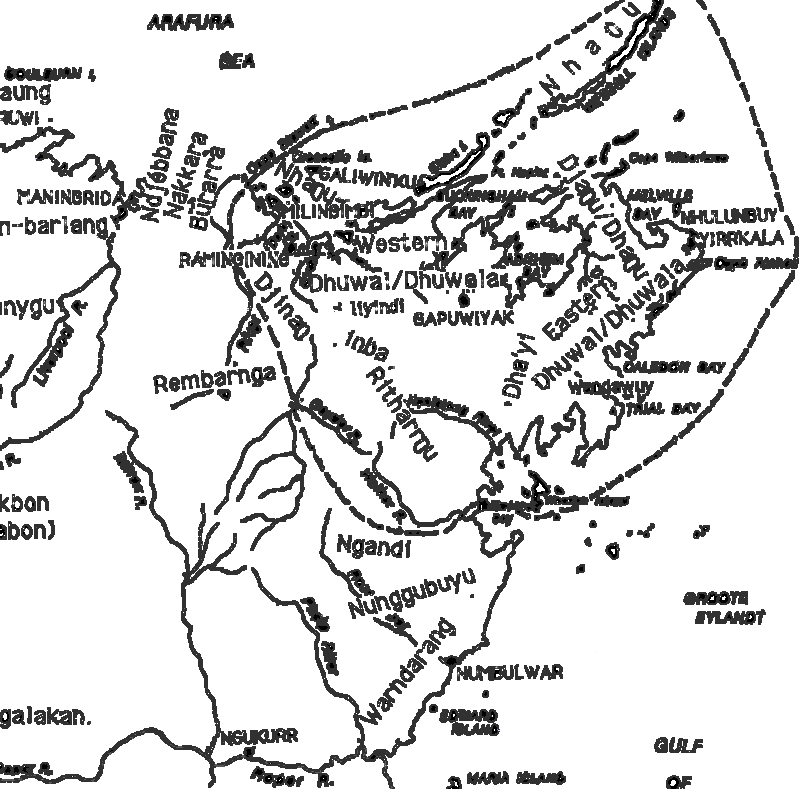
\includegraphics[scale=.2]{YolnguWanga-MW}
\end{columns}
\end{frame}

\begin{frame}{Inflection in Wägilak}
	\begin{itemize}
		\item Heath (1980): Apparent 3-way tense distinction.\\ \textcolor{blue}{\textsc{past}}, \textcolor{forest}{\textsc{present}}, \textcolor{ochre}{\textsc{future}}
		\item Fourth inflection: \textcolor{purple}{\textsc{past potential}}
	\end{itemize}


\only<2>{\begin{tikzpicture}[scale=.9]
	% draw horizontal line   
	\draw[<->, line width=.5mm] (0,0) -- (12,0);
	
	%draw rex
	\fill[gray!10!white] (0,0.02) rectangle (4.8,1.5);
	%	\fill[green!10!white] (2.5,0.02) rectangle (4.8,1.5);
	\fill[blue!10!white] (.02,0.02) rectangle (5,1.5);
	\fill[green!10!white] (5,0.02) rectangle (7,1.5);
	\fill[orange!10!white] (7,0.02) rectangle (12,1.5);
	
	% draw nodes
	%	\draw (1.25,0) node[below=3pt] {\textbf{}} node[above=10pt] {\textsc{\textbf{*}}};
	\draw (2.5,0) node[below=3pt] {\textbf{}} node[above=10pt] {\textbf{\textsc{pst}}};
	%	\draw (5,0)   node[circle,fill,label=below:$\lfloor{\sl today}$] {} node[below=3pt] {\textbf{}} node[above=3pt] {};
	\draw (6,0) node[diamond,shade,inner color=ochre,outer color=black,label=below:$\boldsymbol{t*}$] {} node[below=3pt] {\textbf{}} node[above=3pt] {\textsc{}};
	\draw (6,0) node[below=3pt] {\textbf{}} node[above=10pt] {\textsc{\textbf{pres}}};	
	
	%	\draw (8.25,0) node[below=3pt] {\textbf{}} node[above=10pt] {\textsc{\textbf{I}}};	
	\draw (9.5,0) node[below=3pt] {\textbf{}} node[above=10pt] {\textsc{\textbf{fut}}};	
	%	\draw (9.5,0)   node[circle,fill,label=below:${\sl today}\big)$] {} node[below=3pt] {\textbf{}} node[above=3pt] {};
\end{tikzpicture}}


\only<3>{\begin{columns}
	\column{.5\textwidth}
	\begin{tikzpicture}[scale=.5,font=\footnotesize]
	% draw horizontal line   
	\draw[<->, line width=.5mm] (0,0) -- (12,0);
	
	%draw rex
	\fill[gray!10!white] (0,0.02) rectangle (4.8,1.5);
	%	\fill[green!10!white] (2.5,0.02) rectangle (4.8,1.5);
	\fill[blue!10!white] (.02,0.02) rectangle (5,1.5);
	\fill[green!10!white] (5,0.02) rectangle (7,1.5);
	\fill[orange!10!white] (7,0.02) rectangle (12,1.5);
	
	% draw nodes
%	\draw (1.25,0) node[below=3pt] {\textbf{}} node[above=10pt] {\textsc{\textbf{*}}};
	\draw (2.5,0) node[below=3pt] {\textbf{}} node[above=6pt] {\textbf{\textsc{pst}}};
%	\draw (5,0)   node[circle,fill,label=below:$\lfloor{\sl today}$] {} node[below=3pt] {\textbf{}} node[above=3pt] {};
	\draw (6,0) node[diamond,shade,inner color=ochre,outer color=black,label=below:$\boldsymbol{t*}$] {} node[below=3pt] {\textbf{}} node[above=3pt] {\textsc{}};
	\draw (6,0) node[below=3pt] {\textbf{}} node[above=6pt] {\textsc{\textbf{pres}}};	

%	\draw (8.25,0) node[below=3pt] {\textbf{}} node[above=10pt] {\textsc{\textbf{I}}};	
	\draw (9.5,0) node[below=3pt] {\textbf{}} node[above=6pt] {\textsc{\textbf{fut}}};	
%	\draw (9.5,0)   node[circle,fill,label=below:${\sl today}\big)$] {} node[below=3pt] {\textbf{}} node[above=3pt] {};
\end{tikzpicture}
\column{.5\textwidth}\begin{tikzpicture}
	[scale=1.1,level distance=9mm,
	every node/.style={fill=purple,circle,inner sep=1.5pt},
	level 1/.style={nodes=purple,sibling distance=10mm},
	level 2/.style={sibling distance=8mm},
	level 3/.style={sibling distance=4mm},
	level 4/.style={sibling distance=2mm},
	edge from parent/.style={draw,thick}]
	\node[color=blue] {} [grow=right]
	child {node {} edge from parent[densely dotted,color=purple]
		child {node {}
			child {node {}
				child {node {}}
				child {node {}}}
			child {node {}
				child {node {}}
				child {node {}}}}
		child {node {}
			child {node {}
				child {node {}}
				child {node {}}}
			child {node {}
				child {node {}}
				child {node {}}}}}
	child[missing]
	child {node[color=blue] {}
		child {node {} edge from parent[densely dotted,color=purple]
			child {node {}
				child {node {}}
				child {node {}}}
			child {node {}
				child {node {}}
				child {node {}}}}
		child {node[color=purple] {} edge from parent[densely dotted,color=purple]
			child {node {}
				child {node {}}
				child {node {}}}
			child {node {}
				child {node {}}
				child {node {}}}}
		child {node [style={fill=forest},label=above:$ \boldsymbol{{\color{gray!95}i*}} $] {} []
			child {node[fill=ochre] {} edge from parent[densely dashed,color=ochre,every child=every node\.style={fill=ochre,circle,inner sep=1.5pt}]
				child {node[fill=ochre] {}}
				child {node[fill=ochre] {}}} 
			child {node[fill=ochre] {} edge from parent[densely dashed,color=ochre]
				child {node[fill=ochre] {}}
				child {node[fill=ochre] {}}}} };
\end{tikzpicture}
\end{columns}}
\end{frame}


\subsection{Verbal inflection in Djambarrpuyŋu}
\begin{frame}{\textbf{Yolŋu}\hfill Verbal morphology}
\begin{itemize}
	\item Djambarrpuyŋu: four inflectional categories
	\item Two particular phenomena exhibited in (geographically Western varieties) include:
	\begin{itemize}
		\item \textbf{Cyclic tense} (Comrie 1985)
		\item \textbf{Negative asymmetry} (Miestamo 2005)
	\end{itemize}
	\item Assigning metalinguistic labels to the Djambarrpuyŋu inflectional categories is non-obvious:
	\begin{itemize}
		\item They will be numbered \I, \II, \III, \IV~throughout
		%%% How do they map on to our understanding of TMA catgories
	\end{itemize}
\end{itemize}
\end{frame}


\begin{frame}{\textbf{Distribution of the inflections}}
	\begin{columns}
		\column{0.5\textwidth} 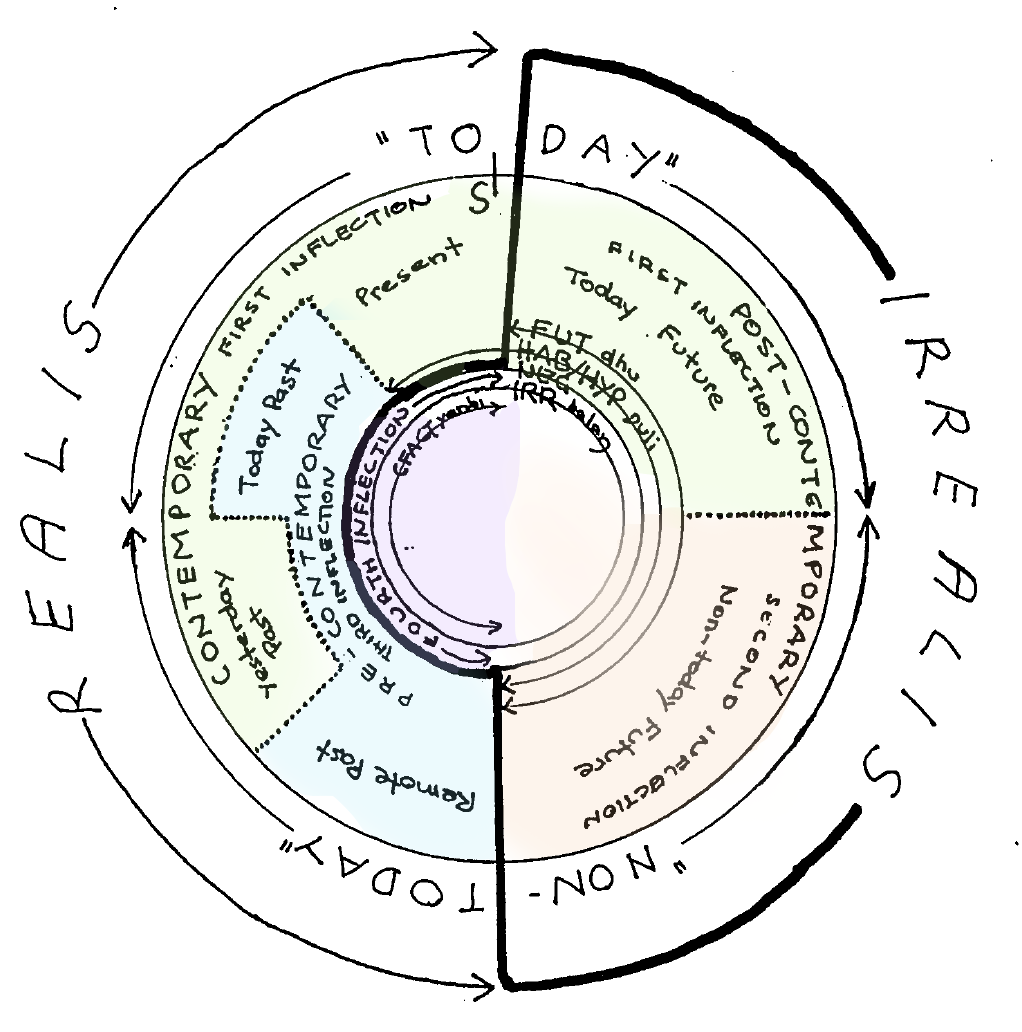
\includegraphics[scale=.2]{../prospectus/WilkinsonDiagram362Col}\scriptsize{(Wilkinson~1991:~362)}
		\column{.5\textwidth}
		\begin{description}
			\item<1->[\I] \textsc{past}, \textsc{present}, \textsc{future}
			\item<2->[\II] \textsc{future}, \textsc{non-past~irrealis}
			\item<3->[\III] \textsc{past}
			\item<4->[\IV] \textsc{past~irrealis, past~habitual}
			\item<5->[$ \star $]  {\color{gray}{here we go...}}
		\end{description}

	\end{columns}
\end{frame}%%ONLY TWO OF THE FOUR ARE AVAILABLE IN IRREALIS SENTENCES (I.E. MIDDLE OF THE CIRCLE)


\begin{frame}{\textbf{Djambarrpuyŋu cyclic tense}}
\begin{itemize}
	\item<1-> Tense morphology licensed by discontinuous intervals
	\item<2> {\small Reported in the languages of Maningrida}
	 \only<2>{\trailingcitation{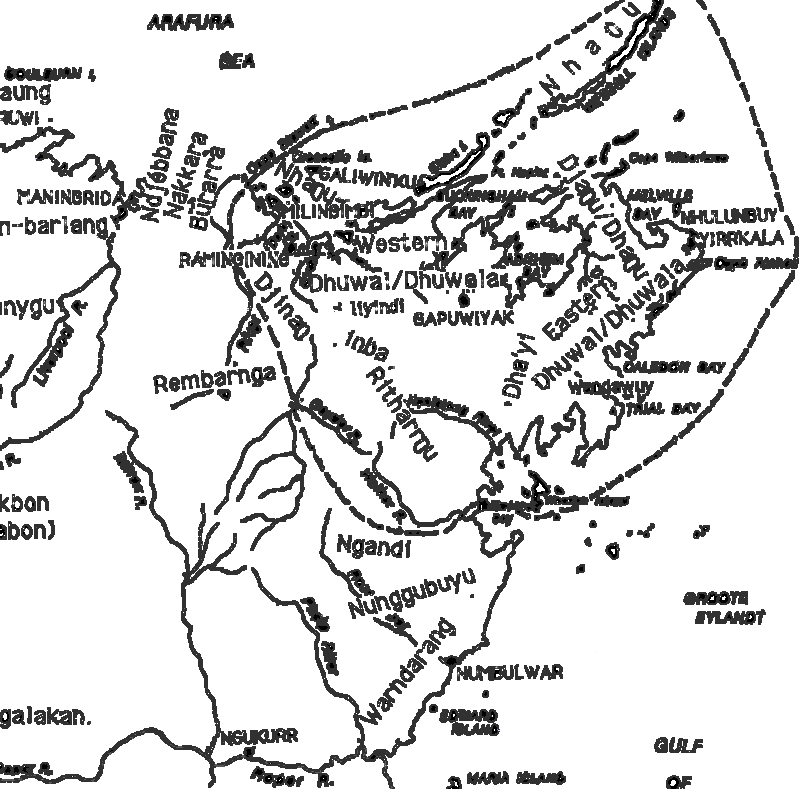
\includegraphics[scale=.2,angle=350]{YolnguWanga-MW}}}


%	\item<3> {\small `Marginal status in the theory on account of its rarity'}
\end{itemize}


	\begin{tikzpicture}[scale=.85]
% draw horizontal line   
\draw[<->, line width=.5mm] (0,0) -- (12,0);



\onslide<8->{	
	\shade[left color=blue!15!white, right color=green!15!white] (0,0.02) rectangle (4.8,1.5);
	\draw (1.25,0) node[below=3pt] {\textbf{}} node[above=10pt] {\textsc{\textbf{III}}};
\draw (3.675,0) node[below=3pt] {\textbf{}} node[above=10pt] {\textbf{I}};}
\onslide<6->{\fill[blue!10!white] (4.8,0.02) rectangle (6.8,1.5); 
	\draw (5.8,0) node[below=3pt] {\textbf{}} node[above=10pt] {\textsc{\textbf{III}}};	}
\onslide<5->{\fill[green!10!white] (6.8,0.02) rectangle (9.5,1.5);
	\draw (8.15,0) node[below=3pt] {\textbf{}} node[above=10pt] {\textsc{\textbf{I}}};	}
\onslide<7->{\fill[orange!10!white] (9.5,0.02) rectangle (12,1.5);
		\draw (10.75,0) node[below=3pt] {\textbf{}} node[above=10pt] {\textsc{\textbf{II}}};	
}

\onslide<3->{\draw (7,0) node[diamond,shade,outer color=black, inner color  = ochre,label=below:$\boldsymbol{t*}$] {} node[below=3pt] {\textbf{}} node[above=3pt] {\textsc{}};}

\onslide<4->{
%draw rex

\draw (5,0)   node[circle,fill,label=below:$\lfloor{\sl today}$] {} node[below=3pt] {\textbf{}} node[above=3pt] {};

\draw (9.5,0)   node[circle,fill,label=below:${\sl today}\big)$] {} node[below=3pt] {\textbf{}} node[above=3pt] {};


}



%%%braces
\onslide<8->{
\draw [decorate,decoration={brace,amplitude=4pt},xshift=-0pt,yshift=35pt]
(0.5,0.5) -- (4.5,0.5) node [black,midway,yshift=0.35cm] 
{\footnotesize metricality};
}

\onslide<9->{
\draw [decorate,decoration={brace,amplitude=4pt},xshift=-0pt,yshift=40pt]
(3.5,0.5) -- (9,0.5) node [black,midway,yshift=0.35cm] 
{\footnotesize cyclicity};}

\end{tikzpicture}
\only<10->{
\textbf{Licensing conditions}

\centering\begin{tabular}{cll}
& $ t_r\circ\text{today} $ & $ t_r\prec\text{today} $\\\midrule
\onslide<9-> 	\I & \textsc{nonpast} & \textsc{recent past} \\
\onslide<10-> \III & \textsc{past} & \textsc{remote past} 
\end{tabular}}

\only<5>{\ex[exno=\bf\it 7]
	\begingl
	\gla ŋarra ga \textbf{nhä-ma} mukulnha//
	\glb 1s \textsc{ipfv}.\I{} \textbf{see}.\I{} aunt.\textsc{acc} yesterday//
	\glft`I'm looking at aunty rn!'//
	\endgl\xe}
\only<6>{\ex[exno=\bf\it 8]
	\begingl
	\gla ŋarra \textbf{nhä-ŋal(a)} mukulnha dhiyaŋ(u)~bili//
	\glb 1s \textbf{see}.\III{} aunt.\textsc{acc} \textsc{prox.erg~cplv}//
	\glft`I saw my aunt just a sec ago'//
	\endgl\xe}
\only<7>{\ex[exno=\bf\it 9]
	\begingl
	\gla ŋarra dhu \textbf{nhä-ŋu} mukulnha goḏarr//
	\glb 1s \textsc{fut} \textbf{see}.\II{} aunt.\textsc{acc} yesterday//
	\glft`I'll see my aunt tomorrow'//
	\endgl\xe}
\only<8>{\ex[exno=\bf\it 10]
	\begingl
	\gla ŋarra \textbf{nhä-ma} mukulnha barpuru//
	\glb 1s \textbf{see}.\I{} aunt.\textsc{acc} yesterday//
	\glft`I saw my aunt yesterday'//
	\endgl\xe}
\only<9>{\ex[exno=\bf\it 11]
	\begingl
	\gla ŋunhi ŋarra yothu yän, ŋarra \textbf{nhä-ŋal(a)} mukulnha//
	\glb \textsc{comp} 1s kid only 1s \textbf{see}.\III{} aunt.\textsc{acc}//
	\glft`I saw my aunty when I was a little kid'//
	\endgl\xe}

\end{frame}

 \setbeamercolor{frametitle}{bg=ochre!50,fg=black}

\section{Negative asymmetry}
\begin{frame}{\transfade \textbf{The negative asymmetry}}
\begin{itemize}
	\item There are a number of overt operators which constrain the distribution of \I~and (particularly) \III~as presented here
	\item<2> \I~ and \III~are ungrammatical under negation
	\end{itemize}

\only<1>{	\begin{tikzpicture}[scale=.85]
% draw horizontal line   
\draw[<->, line width=.5mm] (0,0) -- (12,0);
	
	\shade[left color=blue!15!white, right color=green!15!white] (0,0.02) rectangle (4.8,1.5);
	%	\fill[green!10!white] (2.5,0.02) rectangle (4.8,1.5);
	\fill[blue!10!white] (4.8,0.02) rectangle (6.8,1.5);
	\fill[green!10!white] (6.8,0.02) rectangle (9.5,1.5);
	\fill[orange!10!white] (9.5,0.02) rectangle (12,1.5);
	
	% draw nodes
	\draw (1.25,0) node[below=3pt] {\textbf{}} node[above=10pt] {\textsc{\textbf{III}}};
	\draw (3.675,0) node[below=3pt] {\textbf{}} node[above=10pt] {\textbf{I}};
	
	\draw (5.8,0) node[below=3pt] {\textbf{}} node[above=10pt] {\textsc{\textbf{III}}};	
	\draw (8.15,0) node[below=3pt] {\textbf{}} node[above=10pt] {\textsc{\textbf{I}}};	
	\draw (10.75,0) node[below=3pt] {\textbf{}} node[above=10pt] {\textsc{\textbf{II}}};	
	%draw rex
	
	\draw (5,0)   node[circle,fill,label=below:$\lfloor{\sl today}$] {} node[below=3pt] {\textbf{}} node[above=3pt] {};
	\draw (7,0) node[diamond,shade,outer color=black, inner color  = ochre,label=below:$\boldsymbol{t*}$] {} node[below=3pt] {\textbf{}} node[above=3pt] {\textsc{}};
	\draw (9.5,0)   node[circle,fill,label=below:${\sl today}\big)$] {} node[below=3pt] {\textbf{}} node[above=3pt] {};
\end{tikzpicture}	}

\only<2->{	\begin{tikzpicture}[scale=.85]
% draw horizontal line   
\draw[<->, line width=.5mm] (0,0) -- (12,0);

%draw rex
\shade[left color=RoyalPurple!15!white, right color=orange!15!white] (0,0.02) rectangle (4.8,1.5);
%	\fill[green!10!white] (2.5,0.02) rectangle (4.8,1.5);
\fill[RoyalPurple!10!white] (4.8,0.02) rectangle (6.8,1.5);
\shade[left color=orange!10!white, right color=Green!10!white] (6.8,0.02) rectangle (9.5,1.5);
\fill[orange!10!white] (9.5,0.02) rectangle (12,1.5);

% draw nodes
\draw (1.25,0) node[below=3pt] {\textbf{}} node[above=10pt] {\textsc{\textbf{IV}}};
\draw (3.675,0) node[below=3pt] {\textbf{}} node[above=10pt] {\textbf{II}};
\draw (5,0)   node[circle,fill,label=below:$\lfloor{\sl today}$] {} node[below=3pt] {\textbf{}} node[above=3pt] {};
\draw (7,0) node[diamond,shade,inner color=ochre,outer color=black,label=below:$\boldsymbol{t*}$] {} node[below=3pt] {\textbf{}} node[above=3pt] {\textsc{}};
\draw (5.8,0) node[below=3pt] {\textbf{}} node[above=10pt] {\textsc{\textbf{IV}}};	
\draw (7.5,0) node[below=3pt] {\textbf{}} node[above=10pt] {\textsc{\textbf{II}}};
\draw (9,0) node[below=3pt] {\textbf{}} node[above=10pt] {\textsc{\textbf{I}}};	
\draw (10.75,0) node[below=3pt] {\textbf{}} node[above=10pt] {\textsc{\textbf{II}}};	
\draw (9.5,0)   node[circle,fill,label=below:${\sl today}\big)$] {} node[below=3pt] {\textbf{}} node[above=3pt] {};

\only<3>\path (9,.8) [draw,color=forest,line width=2pt] circle (.9cm);

\end{tikzpicture}	}
\end{frame}


\begin{frame}{\textbf{Asymmetric negation}\hfill Djambarrpuyŋu}\footnotesize


\onslide<1->{\ex[exno=\bf\it 7]
	\begingl
	\gla \rightcomment{\textcolor<1-4>{forest}{\textcolor<5>{ochre}{[\textsc{\textbf{present}}]}}}\only<5>{\textbf{bäyŋu}} ŋarra g\alt<1-4>{a}{i} \textbf<1-4>{nhä\alt{ma}{ŋu}} mukulnha//
	\glb  \only<5>{\textsc{\textbf{nex}}} 1s \textsc{ipfv.\alt<1-4>{\I}{\II}} \textbf{see}.\alt<1-4>{\I}{\II} aunt-\textsc{acc} now//
	\glft`\alt<1-4>{I see my aunt (right now).}{I don't see my aunt (right now).}'//
	\endgl\xe}



\only<2->{\ex[exno=\bf\it8]
	\begingl
	\gla  \rightcomment{\textcolor<1-4>{blue}{{\color<5>{violet}[\textsc{\textbf{today pst}}]}}}\only<5>{\textbf{bäyŋu}} ŋarra \textbf{nhä\alt<1-4>{ŋal}{nha}} mukulnha gäthur//
	\glb \only<5>{\textsc{\textbf{nex}}} 1s \textbf{see}.\alt<1-4>{\III}{\IV}  aunt-\textsc{acc} today//
	\glft`\alt<1-4>{I saw my aunt this morning}{I didn't see my aunt this morning}.'//
	\endgl\xe
	
}

\onslide<3->{\ex[exno=\bf\it 9]
\begingl
	\gla  \rightcomment{\textcolor{ochre}{[\textsc{\textbf{future}}]}}\only<5>{\textbf{bäyŋu}} ŋarra dhu \textbf{nhäŋu} mukulnha//
	\glb  \only<5>{\textsc{\textbf{nex}}} 1s \textsc{fut} \textbf{see}.\II{} aunt.\textsc{acc}//
	\glft`\alt<1-4>{I'll see my aunt (tomorrow).}{I won't see my aunt (tomorrow)}'//
\endgl\xe	}
	
	
\only<4->{\ex[exno=\bf\it10]
\begingl
	\gla \rightcomment{\textcolor<1-4>{forest}{\textcolor<5>{ochre}{[\textsc{\textbf{rec pst}}]}}}\only<5>{\textbf{bäyŋu}} ŋarra \textbf{nhä\alt<1-4>{ma}{ŋu}} mukulnha barpuru//
	\glb \only<5>{\textbf{\textsc{nex}}} 1s \textbf{see}.\alt<1-4>{\I}{\II}  aunt-\textsc{acc} yesterday//
	\glft`\alt<1-4>{I saw my aunt yesterday}{I didn't see my aunt yesterday}.'//
\endgl\xe
}

\end{frame}

\begin{frame}{\textbf{Negative asymmetry}}
%	\begin{itemize}
%		\item Miestamo (2005) presents a typology of \textsc{sentential negation} cross-linguistically
%		\item[\textcolor{Blue}{\textbf{\textsc{defn}}}] Different `reality status marking' in affirmative v. negative sentences\trailingcitation{\footnotesize{(Miestamo~2005)}}
%			\end{itemize}
		\begin{columns}
\column{.5\textwidth}
\textsc{\textbf{\textcolor{Blue}{In Djambarrpuyŋu}}}\\Negative \textsc{realis} and \textsc{irrealis} predications are inflected identically

\column{.5\textwidth}
	\begin{tabular}{ccc}
	&\multicolumn{2}{c}{\textsc{\textbf{inflection}}} \\
	& \textsc{--neg} & \textsc{+neg}\\\midrule
	&	\I & \multirow{2}{*}{\II}\\
	& \II \\\midrule
	&	\III & \multirow{2}{*}{\IV}\\
	& \IV \\\bottomrule
\end{tabular}
		\end{columns}
\end{frame}

%
%\begin{frame}{\textbf{Negative asymmetry}}
%\begin{columns}
%\column{.7\textwidth}
%	\begin{itemize}
%		\item<1-2> Diverges sharply from the Daakie mood system% analysed by Krifka
%		\item<2> Factivity distinction maintained in Daakie, neutralised in \texttt{djr}
%	\end{itemize}
%\column{.3\textwidth}
%
%\begin{tabular}{cc}
%\multicolumn{2}{c}{\textsc{\textbf{Daakie \texttt{[pvo]}}}} \\
%--\textsc{neg} & \textsc{+neg}\\\midrule
%\textsc{\textcolor{forest}{rea$ \oplus $}} & \textsc{\textcolor{ochre}{rea$ \ominus $}}\\
%\textsc{\textcolor{ochre}{pot$ \oplus $}} & \textcolor{ochre}{\textsc{pot$ \ominus $}}\\
%\multicolumn{2}{c}{\textsc{\textcolor{gray!80}{dist}}}
%\end{tabular}
%
%\end{columns}
%\end{frame}

\begin{frame}{\textbf{Negative asymmetry}\hfill\II~and \IV~as \textsc{irr}}
	
\begin{itemize}
	\item So \II~and \IV~turn up as the counterparts of \I~and \III~in negative predication. Also...
\end{itemize}	
	
	\pause
\ex~[exno=\bf\it11]\begingl\gla\rightcomment{\textcolor{ochre}{[\textsc{future}]}}Barpuru goḏarr ŋarra \textbf{dhu} nhä-\textbf{ŋu}//
\glb funeral tomorrow 1s \textsc{\textbf{fut}} see.\II//
\glft `I'll see the funeral tomorrow'//\endgl
\xe
\pause
\ex~[exno=\bf\it 12]\begingl\gla\rightcomment{\textcolor{ochre}{[\textsc{imperative}]}}nhä-\textbf{ŋu} nhanŋu dhurrwara!//
\glb look.{\II} 2s.\textsc{dat} door//
\glft`Look at her mouth!'//\endgl
\xe
\pause

\ex~[exno=\bf\it13]\begingl\gla\rightcomment{\textcolor{ochre}{\textsc{[circ]}}}ŋayi bala \textbf{balaŋu} bakthu-\textbf{rru}//
\glb 3s \textsc{mvtawy} \textsc{\textbf{mod}} break{.\II}//
\glft`It [the recorder] might break.'//\endgl\xe

%\ex\begingl\gla\rightcomment{\textcolor{ochre}{\textsc{[circ $ \lozenge $]}}}Ŋarra \textbf{ŋuli} \textbf{bäynha} dhiŋgun ŋawulul-yu//
%\glb 1s \textsc{mod} \textsc{mod} die.{\II} smoke.\textsc{erg}//
%\glft`I might die from the smoke.'\hfill\scriptsize(Buchanan 78)//\endgl\xe
\end{frame}


\begin{frame}{\textbf{Negative asymmetry}\hfill\II~and \IV~as \textsc{irr}}
%
\ex[exno=\bf\it14]\begingl\gla\rightcomment{\textcolor{violet}{\textsc{[circ]}}}waṯuy \textbf{balaŋu} ḻuka-\textbf{nha} chocolate//
\glb dog.\textsc{erg} \textsc{mod} eat-{\IV} chocolate//
\glft`The dog may/must have eaten the chocolate.'//\endgl\xe
%
\ex[exno=\bf\it15]\begingl\gla\rightcomment{\textcolor{violet}{[\textsc{pst hab}]}}ŋarra \textbf{ŋuli} baman' ḻupḻupthu-\textbf{na} dhiyal//
	\glb 1s \textsc{\textbf{hab}} prior swim-{\IV} \textsc{prox.loc}//
	\glft`I used to swim there.'//\endgl\xe

\ex[exno=\bf\it16]\begingl\gla\rightcomment{\textcolor{violet}{[\textsc{cond}]}}ŋäthil ŋarra \textbf{ŋuli} \textbf{balaŋ} ḻiya-ŋamaŋamayunmi-\textbf{nya} + bala ŋarra \textbf{balaŋ} waŋa-\textbf{nha}-n//
\glb earlier 1sg \textbf{\textsc{mod}} \textbf{\textsc{mod}} head-make.\I.\textsc{refl}-\IV{} then 1s \textsc{\textbf{mod}} speak-\IV-\textsc{seq}//
\glft`Had I thought of it before, I would have spoken.'\trailingcitation{{\scriptsize (Wilk 91)}}//\endgl
\xe 

%
%
\end{frame}

\begin{frame}{\textbf{Negative asymmetry}\hfill\II~and \IV~as \textsc{irr}}
\begin{itemize}

\item \II{} and \IV{} co-occcur with :
\begin{itemize}
	\item \textbf{future} marking 
	\item  \textbf{modals} {\scriptsize (nonepistemic)}
	\item \textbf{negation}
\end{itemize}
	\item Formal treatments of the future predict a range of modal uses of future morphemes 
	\item Compare En. \textit{will} `\textsc{fut}': \textit{that'll be the postman}
\begin{itemize}\small 

	\item ($ \forall $-quantification over different ``conversational bkgrds'')
\end{itemize}
%\item This suggests that they encode irrealis modalities
\item \textbf{Can all this data be unified?}

\end{itemize}
\end{frame}
 
\begin{frame}{\textsc{\textbf{recap}}\hfill \textsc{the paradigms}}
	\begin{columns}[T]
		\column{.45\textwidth}
		
		\textbf{Wägilak}
		\vspace*{1em}
		
			\begin{tikzpicture}[scale=.4,font=\footnotesize]
			% draw horizontal line   
			\draw[<->, line width=.5mm] (0,0) -- (12,0);
			
			%draw rex
			\fill[gray!10!white] (0,0.02) rectangle (4.8,1.5);
			%	\fill[green!10!white] (2.5,0.02) rectangle (4.8,1.5);
			\fill[blue!10!white] (.02,0.02) rectangle (5,1.5);
			\fill[green!10!white] (5,0.02) rectangle (7,1.5);
			\fill[orange!10!white] (7,0.02) rectangle (12,1.5);
			
			% draw nodes
			%	\draw (1.25,0) node[below=3pt] {\textbf{}} node[above=10pt] {\textsc{\textbf{*}}};
			\draw (2.5,0) node[below=3pt] {\textbf{}} node[above=4pt] {\textbf{\textsc{pst}}};
			%	\draw (5,0)   node[circle,fill,label=below:$\lfloor{\sl today}$] {} node[below=3pt] {\textbf{}} node[above=3pt] {};
			\draw (6,0) node[diamond,shade,inner color=ochre,outer color=black,label=below:$\boldsymbol{t*}$] {} node[below=3pt] {\textbf{}} node[above=3pt] {\textsc{}};
			\draw (6,0) node[below=3pt] {\textbf{}} node[above=4pt] {\textsc{\textbf{pres}}};	
			
		
			\draw (9.5,0) node[below=3pt] {\textbf{}} node[above=4pt] {\textsc{\textbf{fut}}};	
		
		\end{tikzpicture}
	
	
		\column{.45\textwidth}
		\textbf{Western Dhuwal(a)}
		
		\textsc{positive}
		\vspace*{.5em}
		
			\begin{tikzpicture}[scale=.4,font=\footnotesize]
			% draw horizontal line   
			\draw[<->, line width=.5mm] (0,0) -- (12,0);
			%		\draw[<-, line width=.5mm] (0,0) -- (9.5,0);	
			%draw rex
			\shade[left color=blue!15!white, right color=green!15!white] (0,0.02) rectangle (4.8,1.5);
			%	\fill[green!10!white] (2.5,0.02) rectangle (4.8,1.5);
			\fill[blue!10!white] (4.8,0.02) rectangle (6.8,1.5);
			\fill[green!10!white] (6.8,0.02) rectangle (9.5,1.5);
			\fill[orange!10!white] (9.5,0.02) rectangle (12,1.5);
			
			% draw nodes
			\draw (1.25,0) node[below=3pt] {\textbf{}} node[above=4pt] {\textsc{\textbf{III}}};
			\draw (3.675,0) node[below=3pt] {\textbf{}} node[above=4pt] {\textbf{I}};
			\draw (5,0)   node[circle,fill] {} node[below=3pt] {\textbf{}} node[above=3pt] {};
			\draw (6.8,0) node[diamond,shade,outer color=black, inner color  = ochre] {} node[below=3pt] {\textbf{}} node[above=3pt] {\textsc{}};
			\draw (5.8,0) node[below=3pt] {\textbf{}} node[above=4pt] {\textsc{\textbf{III}}};	
			\draw (8.15,0) node[below=3pt] {\textbf{}} node[above=4pt] {\textsc{\textbf{I}}};	
			\draw (10.75,0) node[below=3pt] {\textbf{}} node[above=4pt] {\textsc{\textbf{II}}};	
			\draw (9.5,0)   node[circle,fill] {} node[below=3pt] {\textbf{}} node[above=3pt] {};
			
			
			%%%bra
			
		\end{tikzpicture}

		\vspace*{2.5em}
		
		\textsc{negative}	
		\vspace*{.75em}	
		\begin{tikzpicture}[scale=.4,font=\footnotesize]
			% draw horizontal line   
			\draw[<->, line width=.5mm] (0,0) -- (12,0);
			
			%draw rex
			\shade[left color=RoyalPurple!15!white, right color=orange!15!white] (0,0.02) rectangle (4.8,1.5);
			%	\fill[green!10!white] (2.5,0.02) rectangle (4.8,1.5);
			\fill[RoyalPurple!10!white] (4.8,0.02) rectangle (6.8,1.5);
			\shade[left color=orange!10!white, right color=Green!10!white] (6.8,0.02) rectangle (9.5,1.5);
			\fill[orange!10!white] (9.5,0.02) rectangle (12,1.5);
			
			% draw nodes
			\draw (1.25,0) node[below=3pt] {\textbf{}} node[above=4pt] {\textsc{\textbf{IV}}};
			\draw (3.675,0) node[below=3pt] {\textbf{}} node[above=4pt] {\textbf{II}};
			\draw (5,0)   node[circle,fill] {} node[below=3pt] {\textbf{}} node[above=3pt] {};
			\draw (7,0) node[diamond,shade,inner color=ochre,outer color=black] {} node[below=3pt] {\textbf{}} node[above=3pt] {\textsc{}};
			\draw (5.8,0) node[below=3pt] {\textbf{}} node[above=4pt] {\textsc{\textbf{IV}}};	
			\draw (7.5,0) node[below=3pt] {\textbf{}} node[above=4pt] {\textsc{\textbf{II}}};
			\draw (9,0) node[below=3pt] {\textbf{}} node[above=4pt] {\textsc{\textbf{I}}};	
			\draw (10.75,0) node[below=3pt] {\textbf{}} node[above=4pt] {\textsc{\textbf{II}}};	
			\draw (9.5,0)   node[circle,fill] {} node[below=3pt] {\textbf{}} node[above=3pt] {};
		
			
	\end{tikzpicture}

	\end{columns}
\end{frame}


\section{An irrealis semantics}



%\begin{frame}{\textbf{Modal particles}}
%	\begin{itemize}
%	%		\item In Wägilak, future morphemes have additional modal necessity uses
%		\item In WD, the irrealis categories (\II~\& \IV) always* co-occur in some with a marker of:
%		\begin{itemize}
%			\item \textsc{futurity} (\textit{dhu})
%			\item \textsc{(circ) modality} (incl. conditionals) (\textit{balaŋu, ŋuli})
%			\item \textsc{negation} (\textit{yaka, bäyŋu})	
%		\end{itemize} 
%	\end{itemize}
%\end{frame}

\begin{frame}{\textbf{Negation as a modal operator}}
	\begin{itemize}
%		\item These can be treated as a natural class insofar as they mark \textbf{non-realised} eventualities
		\item<1-> Building on a symbolic-logical tradition that conceives of negation as a modal operator\\
		 \textbf{Negation as a (species of) alethic impossiblity}\hfill(cf {\small Wansing 2001}):$$\mathcal M,w\vDash\sim A\iff \forall u.w\mathbb C u\to\mathcal M,u\not\vDash A$$
%		 \textsc{in words.} a world verifies the...
		 
		\item<2-> I propose that \textit{yaka, bäyŋu} \textsc{`neg'} are part of a class of modal particles (2-place operators, following Kratzer a.o.)
		
			 $$ \denote{\textsc{neg}} = \lambda P_{\langle s,t\rangle}\lambda w. \nexists w^\prime[w^\prime\in\cap\mathbb C(w)\to\textsc{at}(P,w^\prime)] $$
			 
			{\small Pred modifiers that asserts that there's no $ w $-compatible world, the pred is not instantiated\\
			 \textit{I.e.}, they effectively mark the counterfactual status of $ P $}
			 
		\item<3-> Takeaway: there's a way of conceptualising $ \neg $ as a (2-place) modal operator
\end{itemize}\end{frame}
\begin{frame}{\textbf{Modal particles}}
		
	\begin{itemize}	
			\item This treatment allows us to posit a natural class with the other licensing environments for \II~and \IV.\pause
			\item In one way or another, WD modal particles signal the \textbf{objective nonveridicality} of prejacent
			\begin{itemize}
				\item $\underset{\text{def}}{=} \exists w^\prime[w^\prime\in\mathbb M\wedge w^\prime\in\neg p]$\hspace{2in}\footnotesize (Giannakidou 2016a.o.)
				\item this p much means that \textbf{the truth of a given proposition can't be known/asserted} as a ``settled'' fact in a given situation
			\end{itemize}
			\item Our semantics for negative and modal operators --- those elements that co-occur with \II~and \IV~--- all satisfy \textbf{nonveridicality} in some circumstantial modal base
	\end{itemize}
\end{frame}


%todo generalization
%	\item \textbf{In Djambarrpuyŋu}:
%
%\begin{itemize}
% \textsc{irrealis categories} (\II{} and \IV{}) have generalised -- they mark nonrealised eventualities
%\item \textbf{This gives rise to the negative asymmetry}\pause
%\item Cyclic tense: \II~ presupposes a nonrealised event where $ \I\big(t*,t_e\big) $
%\item Preverbal particles constrain quantificational domains\\
%\textit{yaka/bäyŋu} `\textsc{neg}', \textit{balaŋu} `\textsc{mod}', \textsc{dhu} `\textsc{fut}'...		\end{itemize}



%\begin{itemize}	\item
%	 \deftagex{dhu-sems}$ \denote{\textit{dhu}}=\lambda o\lambda m\lambda P\lambda i:\forall b\ni i\big[b\in\underset{o}{\textsc{best}}\big(\underset{\textsc{circ}}{\cap m(i)}\big)\to\exists i^\prime\in b[i^\prime\succeq i\wedge \textsc{at}(P,i)]\big] $
%	\item \deftagex{balaŋ-sems}
%	$ \denote{\textit{balaŋ(u)}} = \lambda o\lambda m\lambda P\lambda i.\exists b\ni i'\big[b\in\underset{o}{\textsc{best}}\big(\underset{\textsc{circ}}{\cap m(i)}\big)\wedge\exists i'\succeq i\wedge \textsc{at}\big(P,i)\big]$
%\end{itemize}
%\end{frame}
\begin{frame}{\II~and \IV~as \textsc{irrealis} mood}
%\begin{columns}
%\column{.6\textwidth}

	\begin{itemize}
		\item<1-> suggests a treatment of WD inflections as verbal mood
		\item<2-> super dissimilar to the \textsc{ind-sbjv} distinction in European
		\begin{itemize}
			\item<3-> \textsc{not} licensed by subordinating preds \item<4-> Also not licensed by \textbf{epistemic modals}
			
%			\only<4>{\pex\begingl\gla je veux q\xe}
		\end{itemize}
	\item<4-> Paradigm realises a systematic \textsc{realis-irrealis} distinction
	\begin{itemize}
		\item this notion is both much-used and much-maligned in the typological literature
		\item Krifka, von Prince \textit{et al.} have formal proposals in \textsc{n/c-}vanuatuan langs
	\end{itemize}
	\end{itemize}
%\column{.4\textwidth}
%\end{columns}
\end{frame}
\begin{frame}{\textbf{Proposal for the WD paradigm}}
	\begin{columns}
% TODO: \usepackage{graphicx} required
\column{.5\linewidth}
The paradigm is organised around two semantic features:
\begin{itemize}
	
	
		\item \textsc{Nonveridicality}\\%}\\(or ``ahistoricity'')}
	\only<2->{{\scriptsize satisfied~when~c-commanding~a~modal}}
	{{\color{gray!120}\small$$\exists i^\prime[i^\prime\in\cap\approx_i\wedge P(i^\prime)]$$}}


	\item<3-> \textsc{``Precontemporaneity'' (nonfinal instantiation)}
	{{\color{gray}\small$$\exists j[j\underset{\textsc{final}}{\sqsubseteq} i\wedge
%		\exists k [k\sqsubseteq j\wedge k\prec i\wedge P(k)]]$$}
		\textsc{NfInst}(P,i,j)]\trailingcitation{\scriptsize{(C\&D '15)}}$$}}

	
\end{itemize}\pause
\column{.5\linewidth}\begin{center}
	\only<4->{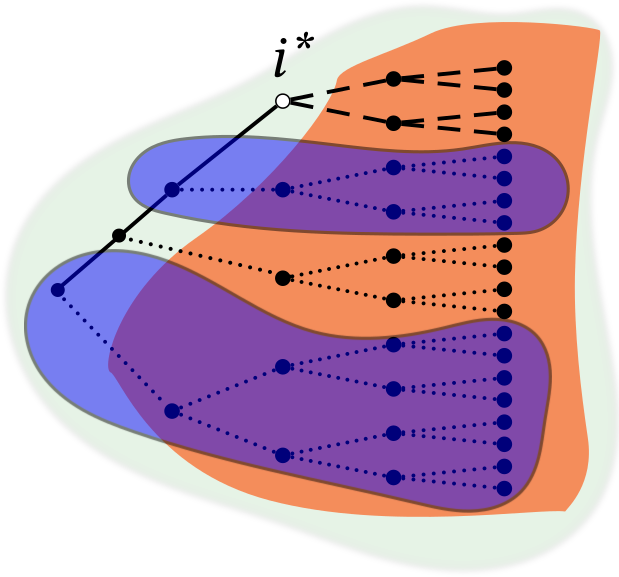
\includegraphics[width=.9\linewidth]{infldomains}
	
	{\large\I\hfill\II\hfill\III\hfill\IV}}
\end{center}
\end{columns}
\end{frame}



%\begin{frame}{\textbf{Proposal for the WD paradigm}}
%	\begin{columns}
%		% TODO: \usepackage{graphicx} required
%		\column{.5\linewidth}
%	\begin{itemize}
%	\item 	\textbf{\textsc{Nonveridicality}} is a presupposition of the inflection
%	\item it's satisfied when there is a \textsc{modal} element (incl. negation) in its c-command domain
%					
%		\end{itemize}
%		\column{.4\linewidth}\begin{center}
%			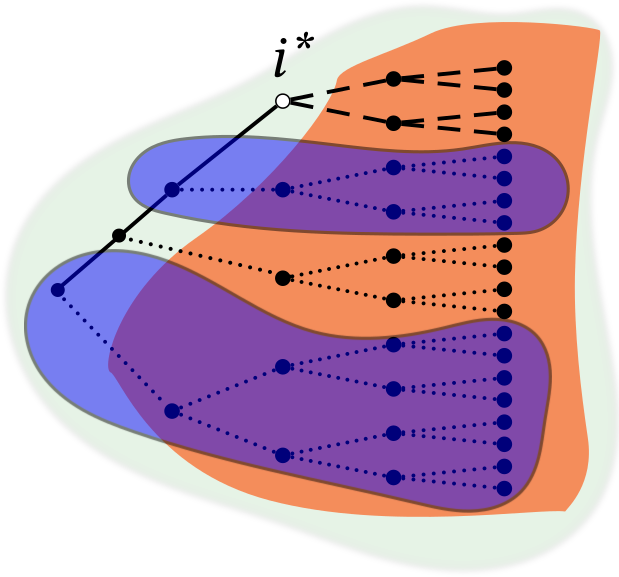
\includegraphics[width=.9\linewidth]{infldomains}
%			
%			{\large\I\hfill\II\hfill\III\hfill\IV}
%		\end{center}
%	\end{columns}
%\end{frame}


\begin{frame}{\textbf{Proposal for the WD paradigm}}
	\begin{columns}
		% TODO: \usepackage{graphicx} required
		\column{.7\linewidth}
\only<2>{\footnotesize$\denote[i*]{\I} =\lambda P\lambda i.P(i) $ \\[1em]
	$\denote[i*]{\II} =\lambda P\lambda i:\textcolor{Apricot}{\exists i{^\prime}[i{^\prime}\in\cap\approx_{i}\wedge\neg P(i{^\prime})\big]}.P(i) $\\[1em]
	$\denote[i*]{\III} = \lambda P\lambda i:\textcolor{Mahogany}{\exists j[j\underset{\textsc{final}}{\sqsubseteq} i.\textsc{NfInst}(P,i,j)]}$\\[1em]
	$\begin{aligned}\denote[i*]{\IV}  = \lambda P\lambda i:\textcolor{Apricot}{\exists i{^\prime}[i{^\prime}\in\cap\approx_{i}\wedge\neg P(i{^\prime})\big]}\wedge\textcolor{Mahogany}{\exists j[j\underset{\textsc{final}}{\sqsubseteq} i.\textsc{NfInst}(P,i,j)]}\end{aligned}$}
\only<1>{\Large\centering \begin{tabular}[t]{>{\columncolor{gray!20}} ccc}
		\rowcolor{gray!20}	&	\textminus\textsc{nonver} & \textsc{+nonver}\\%\midrule
		\textminus\textsc{Precon}& \I&\II \\
		\textsc{+Precon}& \III & \IV
	\end{tabular}}
		\column{.3\linewidth}
			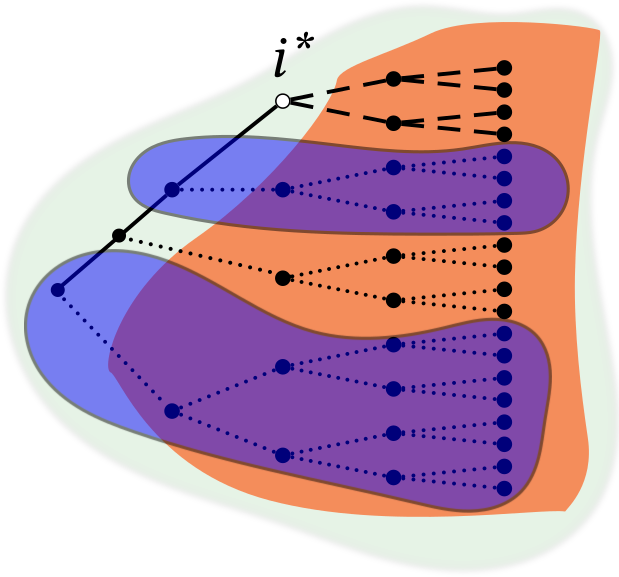
\includegraphics[width=1.1\linewidth]{infldomains}
			\begin{center}
			{\large\I\hfill\II\hfill\III\hfill\IV}
		\end{center}
	\end{columns}
\end{frame}

 \setbeamercolor{frametitle}{bg=YellowGreen!50,fg=black}
\section*{Appendices}
\begin{frame}{\textbf{\textsc{Conclusions}}}
	\begin{itemize}
		\item<+-> We've seen a treatmenet of negative operators that places them in a class of modals
		\item<+-> We've seen how the interaction of two properties--- \textsc{nonveridicality} and \textsc{precontemporaneity }---get us a principled analysis of WD inflectional semantics (\I, \II, \III, \IV)
		\item<+-> {\small (see dissertation for intricacies \& semantic composition)}
	\end{itemize}
\end{frame}



%%% options: back to Krifka? Negation as a modal operator? Why this works why it's motivated? How this can capture diacrhrony
%% Wägilak, no asymmetry, decently strightforward tense semantics
% why diachrony can be useful for discussing competing synchronic analyses, how can we get from one to the other, richer theoretical undersgtanding of L.)
% envoi: other complexities -- is this a tenseless system?  spruik/fanfic my dissertation, openish Qs(???)
% appendix about directionalrty (proto-Yolŋu system, foreshadow this.)



\begin{frame}{\textbf{Selected References}}\footnotesize
 \textbf{Bhat} (1999) \textit{Prominence of Tense, Mood \& Aspect} • \textbf{Boneh} (2016) On becoming a tense prominent system. \textit{FoDS1} • \textbf{Bowern} (2009) Conjugation class stability. \textit{ICHL19} • \textbf{Bybee, Perkins \& Pacuglia }(1991) \textit{Evolution of Grammar} • \textbf{Comrie} (1985) \textit{Tense} • \textbf{Condoravdi} (2002) Temporal Interpretation of Modals • \textbf{Condoravdi \& Deo} (2014) Aspect shifts in Indo-Aryan and trajectories of semantic change • \textbf{Copley} (2009) \textit{The semantics of the Future} • \textbf{Giannikidou} (2016). Evaluative subjunctive and nonveridicality • \textbf{de Haan} (2012) Irrealis: fact or fiction? \textit{Lang. Sci. 34} • \textbf{Heath} (1981) \textit{Ritharrŋu} •  \textbf{Kaufmann} (2005) Conditional truth and future reference • \textbf{---, Condoravdi \& Harizanov} (2006) Formal approaches to modality • \textbf{Krazer} (1989) Lumps of thought \textit{L\&P} • \textbf{Krifka} (2016) Realis \& nonrealis modalities in Daakie. \textit{SALT26} • \textbf{Lowe} (n.d.) \textit{Grammar lessons in Gupapuyŋu} • \textbf{Matthewson} (2010) Cross-linguistic variation in modality systems: The role of mood. \textit{S\&P} • \textbf{Miestamo} (2005) \textit{Standard negation} •\textbf{ von Prince }(2019) Counterfactuality and past. \textit{L\&P} • \textbf{Ripley} (2009) \textit{Negation in natural language} • \textbf{Thomason} (1970) Indeterminist time and truth-value gaps • \textbf{Waters} (1989) \textit{Djinang \& Djinba} • \textbf{Wansing} (2001) Negation. \textit{Blackwell Phil. Logic} • \textbf{Wilkinson} (1991) \textit{Djambarrpuyŋu}.

%	\bibliography{FullBiblio.bib}
\end{frame}
\subsection*{Same-day future}

\begin{frame}{\textbf{Appendix A}\hfill The \I{} same-day future}

\only<1>{
		\begin{tikzpicture}[scale=.85]
	% draw horizontal line   
	\draw[<->, line width=.5mm] (0,0) -- (12,0);
		
		\shade[left color=blue!15!white, right color=green!15!white] (0,0.02) rectangle (4.8,1.5);
		%	\fill[green!10!white] (2.5,0.02) rectangle (4.8,1.5);
		\fill[blue!10!white] (4.8,0.02) rectangle (6.8,1.5);
		\fill[green!10!white] (6.8,0.02) rectangle (9.5,1.5);
		\fill[orange!10!white] (9.5,0.02) rectangle (12,1.5);
		
		% draw nodes
		\draw (1.25,0) node[below=3pt] {\textbf{}} node[above=10pt] {\textsc{\textbf{III}}};
		\draw (3.675,0) node[below=3pt] {\textbf{}} node[above=10pt] {\textbf{I}};
		
		\draw (5.8,0) node[below=3pt] {\textbf{}} node[above=10pt] {\textsc{\textbf{III}}};	
		\draw (8.15,0) node[below=3pt] {\textbf{}} node[above=10pt] {\textsc{\textbf{I}}};	
		\draw (10.75,0) node[below=3pt] {\textbf{}} node[above=10pt] {\textsc{\textbf{II}}};	

		\draw (5,0)   node[circle,fill,label=below:$\lfloor{\sl today}$] {} node[below=3pt] {\textbf{}} node[above=3pt] {};
		\draw (7,0) node[diamond,shade,outer color=black, inner color  = ochre,label=below:$\boldsymbol{t*}$] {} node[below=3pt] {\textbf{}} node[above=3pt] {\textsc{}};
		\draw (9.5,0)   node[circle,fill,label=below:${\sl today}\big)$] {} node[below=3pt] {\textbf{}} node[above=3pt] {};
				\end{tikzpicture}	
						}	


	\only<2->{	\begin{tikzpicture}[scale=.85]
		% draw horizontal line   
		\draw[<->, line width=.5mm] (0,0) -- (12,0);
		
		%draw rex
		\shade[left color=RoyalPurple!15!white, right color=orange!15!white] (0,0.02) rectangle (4.8,1.5);
		%	\fill[green!10!white] (2.5,0.02) rectangle (4.8,1.5);
		\fill[RoyalPurple!10!white] (4.8,0.02) rectangle (6.8,1.5);
		\shade[left color=orange!10!white, right color=Green!10!white] (6.8,0.02) rectangle (9.5,1.5);
		\fill[orange!10!white] (9.5,0.02) rectangle (12,1.5);
		
		% draw nodes
		\draw (1.25,0) node[below=3pt] {\textbf{}} node[above=10pt] {\textsc{\textbf{IV}}};
		\draw (3.675,0) node[below=3pt] {\textbf{}} node[above=10pt] {\textbf{II}};
		\draw (5,0)   node[circle,fill,label=below:$\lfloor{\sl today}$] {} node[below=3pt] {\textbf{}} node[above=3pt] {};
		\draw (7,0) node[diamond,shade,inner color=ochre,outer color=black,label=below:$\boldsymbol{t*}$] {} node[below=3pt] {\textbf{}} node[above=3pt] {\textsc{}};
		\draw (5.8,0) node[below=3pt] {\textbf{}} node[above=10pt] {\textsc{\textbf{IV}}};	
		\draw (7.5,0) node[below=3pt] {\textbf{}} node[above=10pt] {\textsc{\textbf{II}}};
		\draw (9,0) node[below=3pt] {\textbf{}} node[above=10pt] {\textsc{\textbf{I}}};	
		\draw (10.75,0) node[below=3pt] {\textbf{}} node[above=10pt] {\textsc{\textbf{II}}};	
		\draw (9.5,0)   node[circle,fill,label=below:${\sl today}\big)$] {} node[below=3pt] {\textbf{}} node[above=3pt] {};
		
\path (9,.8) [draw,color=forest,line width=2pt] circle (.9cm);
				\end{tikzpicture}

\begin{itemize}
	\item Under negation, \I~occurs only in same-day future predications
\end{itemize}

\pex[exno=\bf\it17]
\begingl\gla\rightcomment{\textbf{\textsc{\textcolor{forest}{[same-day fut]}}}}(bäyŋu) ŋarra dhu~ga ŋhä\textbf{ma} mukulnha//
\glb (\textsc{neg}) 1s \textsc{fut}~\textsc{ipfv}.{\I} see.{\I} aunty.\textsc{acc}//
\glft`I'm (not) seeing my aunt (tonight).'\endgl//
\xe
}
\end{frame}

\begin{frame}{\textbf{Appendix \textsc{a}}\hfill The \I{} same-day future}
	\begin{itemize}
		\item A grammaticalised \textsc{futurate}\hfill{\scriptsize (Copley 2009)}
		$$ \textsc{plan}(d)(p)(w)(t) $$
		\item `The speaker of a futurate has some high level of confidence that the future eventuality will happen'
		\item Copley's conditional presupposition: \textit{If $ p $ is planned, $ p $ will happen}
		\item In this case, the reality status of $ \textsc{plan}(p) $ and $ \textsc{plan}(\neg p) $ ought to be the same.
	\end{itemize}
\end{frame}


\begin{frame}{\textbf{Appendix \textsc{a}}\hfill The \I{} same-day future}
	\begin{itemize}
		\item Conversely the neutralisation still happens in the present

	\onslide<1->{\ex[exno=\bf\it 7]
		\begingl
		\gla \rightcomment{\textcolor<1>{forest}{\textcolor<2>{ochre}{[\textsc{\textbf{present}}]}}}\only<2>{\textbf{bäyŋu}} ŋarra g\alt<1>{a}{i} \textbf<1>{nhä\alt{ma}{ŋu}} mukulnha//
		\glb  \only<2>{\textsc{\textbf{nex}}} 1s \textsc{ipfv.\alt<1>{\I}{\II}} \textbf{see}.\alt<1>{\I}{\II} aunt-\textsc{acc} now//
		\glft`\alt<1>{I see my aunt (right now).}{I don't see my aunt (right now).}'//
		\endgl\xe}
	\item Negative present descriptions are still counterfactual
	\item Note that this is fine for the current analysis:\\\I~is maximially underspecified, and is outcompeted by the other inflections \textsc{(MaxPresupp)}
		\end{itemize}
\end{frame}

%	\subsection*{\textbf{Appendix \textsc{b}}\hfill Epistemics and attitudes}
%	\begin{frame}{Propositional attitudes}
%	\begin{itemize}
%		\item I'd pointed out that the semantics of higher predicate doesn't license \textsc{irr} (\textit{contra} \textsc{sbjv})
%		
%		
%		
%		
%	\end{itemize}
%\end{frame}

\subsection*{Directionality}
\begin{frame}{\textbf{Appendix C}\hfill Directionality}
\begin{itemize}
	\item Yolŋu as a Pama-Nyungan ``enclave'' in the Arnhem Land
	\item Most other (nPN) Arnhem languages express \textsc{neg} asymmetry
	\item Maningrida language family has cyclic tense
	\item Waters (1989) provides a number of other features shared between W Yolŋu and Arnhem languages
	\item Evidence of a Sprachbund
	\item Bowern (2009) proposes a 6-way inflected Proto-Yolŋu paradigm. The West Arnhem Sprachbund features are not reconstructed.\end{itemize}
\end{frame}





\subsection*{Wägilak}

\begin{frame}{\textbf{Appendix D\hfill Inflection in Wägilak}}
	
	\ex\begingl\gla \rightcomment{\textcolor{ochre}{\textbf{[\textsc{future}]}}}goḏarr ŋarra \textbf<1>{nhäŋu}\only<2>{\textbf{-'ma'}} mukulnha//
	\glb tomorrow 1s see.\II{}\only<2>{-\textsc{\textbf{neg}}} aunt.\textsc{acc}//
	\glft`I \alt<1>{will}{won't} see my aunt tomorrow.'//\endgl\xe
	
	\ex\begingl\gla \rightcomment{\textcolor{forest}{\textbf{[\textsc{present}]}}}\textbf<1>{nhäma}\only<2>{\textbf{-'ma'}} rra yakuthi mukulnha//
	\glb see.\textbf{{\I}}\only<2>{-\textsc{\textbf{neg}}} 1s now aunt.\textsc{acc}//
	\glft`I'm \only<2>{(not)} looking at my aunt currently.'//\endgl\xe
	
	
	\ex\begingl\gla \rightcomment{\textcolor{blue}{\textbf{[\textsc{past}]}}}gätha ŋarra \textbf<1>{nhäwala}\only<2>{\textbf{-'ma'}} mukulnha//
	\glb today 1s see.\textbf{\III}\only<2>{-\textsc{\textbf{neg}}} aunt.\textsc{acc}//
	\glft`I \alt<1>{saw}{didn't see} my aunt this morning.'//\endgl
	\xe
\end{frame}


\begin{frame}{\textbf{Appendix C\hfill Inflection in Wägilak}}
	\begin{itemize}
		\item Closest related Yolŋu languages do not exhibit the asymmetry
		\item Inflections encode temporal information
		\item Imperatives formally identical to declaratives
		\item \II~and \IV~ also occur in conditionals (without modal particles)
	\end{itemize}
	
	
	\ex \begingl\gla \rightcomment{\textcolor{violet}{\textbf{[\textsc{sbjv}]}}}\textbf{wäniya} ŋay ŋunbalaya bulu, ŋayi \textbf{guyupiya}//
	\glb go.\IV{} 3s that~way again 3s die.\IV//
	\glft`If he had gone that way, he would've died'//\endgl\xe
	
	
	\ex \begingl\gla \rightcomment{\textcolor{ochre}{\textbf{[\textsc{cond}]}}}\textbf{wäni} ŋay ŋunbalaya bulu, ŋayi \textbf{guyupi}//
	\glb go.\II{} 3s that~way again 3s die.\II//
	\glft`If he had gone that way, he would've died'//\endgl\xe
	
	
\end{frame}
\end{document}

\begin{frame}{Appendix D\hfill \textbf{Wägilak}\hfill\II~and \IV~as \textsc{irr}}
	\begin{itemize}
		\item We need a way of uniting the \textsc{future} and \textsc{modal} (e.g. conditional) uses of \II
		\item \II{} as a \textsc{modal for the present}
		
		
		$$\llbracket\II(\varphi)\rrbracket^{w,t*,\textbf{\textsc{mb}}}\leftrightarrow\forall w^\prime\in \textsc{\textbf{mb}}(w,t*)[t*\preceq t^\prime\wedge\varphi(w^\prime,t^\prime)] $$
		
		
		\item \IV{} as a \textsc{modal for the past}		
		
		$$\llbracket\IV(\varphi)\rrbracket^{w,t*,\textbf{\textsc{mb}}}\leftrightarrow\forall w^\prime\in \textsc{\textbf{mb}}(w,t*)[t*\succ t^\prime\wedge\varphi(w^\prime,t^\prime)] $$
	\end{itemize}
	
\end{frame}



